\documentclass[11pt, a4paper]{article}
\usepackage{pdfpages}
\usepackage{parallel}
\usepackage[T2A]{fontenc}
%\usepackage{ucs}
\usepackage[utf8]{inputenc}
\usepackage[english,russian]{babel}
\usepackage{hyperref}
\usepackage{rotating}
\usepackage[inner=2cm,top=1.8cm,outer=2cm,bottom=2.3cm,nohead]{geometry}
%\usepackage{listings}
\usepackage{graphicx}
\usepackage{wrapfig}
\usepackage{longtable}
\usepackage{indentfirst}
\usepackage{array}
\usepackage{tikzsymbols}
\usepackage{soul}
\usepackage[ruled,vlined]{algorithm2e}
\usepackage{qrcode}
\counterwithout{figure}{section} 

\usepackage{url}
\makeatletter
\g@addto@macro{\UrlBreaks}{\UrlOrds}
\makeatother

\newcolumntype{P}[1]{>{\raggedright\arraybackslash}p{#1}}
\frenchspacing
%\usepackage{fixltx2e} %text sub- and superscripts
\usepackage{icomma} % коскі ў матэматычным рэжыме
%\PreloadUnicodePage{4}

\newcommand{\longpage}{\enlargethispage{\baselineskip}}
\newcommand{\shortpage}{\enlargethispage{-\baselineskip}}

\def\switchlang#1{\expandafter\csname switchlang#1\endcsname}
\def\switchlangbe{
\let\saverefname=\refname%
\def\refname{Літаратура}%
\def\figurename{Іл.}%
}
\def\switchlangru{
\let\saverefname=\refname%
\let\savefigurename=\figurename%
\def\refname{Литература}%
\def\figurename{Рис.}%
}
\def\switchlangen{
\let\saverefname=\refname%
\def\refname{References}%
\def\figurename{Fig.}%
}

\hyphenation{admi-ni-stra-tive}
\hyphenation{ex-pe-ri-ence}
\hyphenation{fle-xi-bi-li-ty}
\hyphenation{Py-thon}
\hyphenation{ma-the-ma-ti-cal}
\hyphenation{re-ported}
\hyphenation{imp-le-menta-tions}
\hyphenation{pro-vides}
\hyphenation{en-gi-neering}
\hyphenation{com-pa-ti-bi-li-ty}
\hyphenation{im-pos-sible}
\hyphenation{desk-top}
\hyphenation{elec-tro-nic}
\hyphenation{com-pa-ny}
\hyphenation{de-ve-lop-ment}
\hyphenation{de-ve-loping}
\hyphenation{de-ve-lop}
\hyphenation{da-ta-ba-se}
\hyphenation{plat-forms}
\hyphenation{or-ga-ni-za-tion}
\hyphenation{pro-gramming}
\hyphenation{in-stru-ments}
\hyphenation{Li-nux}
\hyphenation{sour-ce}
\hyphenation{en-vi-ron-ment}
\hyphenation{Te-le-pathy}
\hyphenation{Li-nux-ov-ka}
\hyphenation{Open-BSD}
\hyphenation{Free-BSD}
\hyphenation{men-ti-on-ed}
\hyphenation{app-li-ca-tion}

\def\progref!#1!{\texttt{#1}}
\renewcommand{\arraystretch}{2} %Іначай формулы ў матрыцы зліпаюцца з лініямі
\usepackage{array}

\def\interview #1 (#2), #3, #4, #5\par{

\section[#1, #3, #4]{#1 -- #3, #4}
\def\qname{LVEE}
\def\aname{#1}
\def\q ##1\par{{\noindent \bf \qname: ##1 }\par}
\def\a{{\noindent \bf \aname: } \def\qname{L}\def\aname{#2}}
}

\def\interview* #1 (#2), #3, #4, #5\par{

\section*{#1\\{\small\rm #3, #4. #5}}
\ifx\ParallelWhichBox\undefined%
    \addcontentsline{toc}{section}{#1, #3, #4}%
\else%
\ifnum\ParallelWhichBox=0%
    \addcontentsline{toc}{section}{#1, #3, #4}%
\fi\fi%

\def\qname{LVEE}
\def\aname{#1}
\def\q ##1\par{{\noindent \bf \qname: ##1 }\par}
\def\a{{\noindent \bf \aname: } \def\qname{L}\def\aname{#2}}
}

\newcommand{\interviewfooter}[1]{
\vskip 1em
\noindent \textit{#1}
}

\AtEndDocument{\vfill\centering \qrcode{https://github.com/fiowro/mouses/blob/main/\jobname.pdf}}

\switchlang{ru}
\begin{document}

\title{1988 "--- Asher Turbo trackball}
\date{}
\maketitle
\selectlanguage{russian}
Трекбол Asher Turbo, показанный на рис. \ref{fig:AsherPic}, является устройством для компьютеров Apple Macintosh с шиной ADB, разработанным на базе трекбола quadLynx "--- разновидности семейства трекболов LX200. Трекболы LX200, более известные своими вариантами microLYNX и comLYNX, были выпущены в калифорнии компанией Honeywell, дуочерним предприятием Disc Instruments; это семейство оказалось долгожителем и в дальнейшем выдержало множество переизданий под разными брэндами, отличаясь интерфейсом подключения и блоком электроники \cite{lx200}. Рекламные материалы позволяют датировать модель quadLYNX под брэндом Honeywell 1986 годом \cite{honeywell}. А в 1988 году под брэндом Asher Engineering Corporation появляется два трекбола: quadLYNX <<LX200-192-D1>> (с упоминанием Honeywell в качестве изначального разработчика устройства) \cite{asher} и Turbo Trackball <<LX200-192-S3A>>, в корпусе другой формы, но с сильным сходством в части внутренних конструктивных решений \cite{turbo}.

\begin{figure}[h]
    \centering
    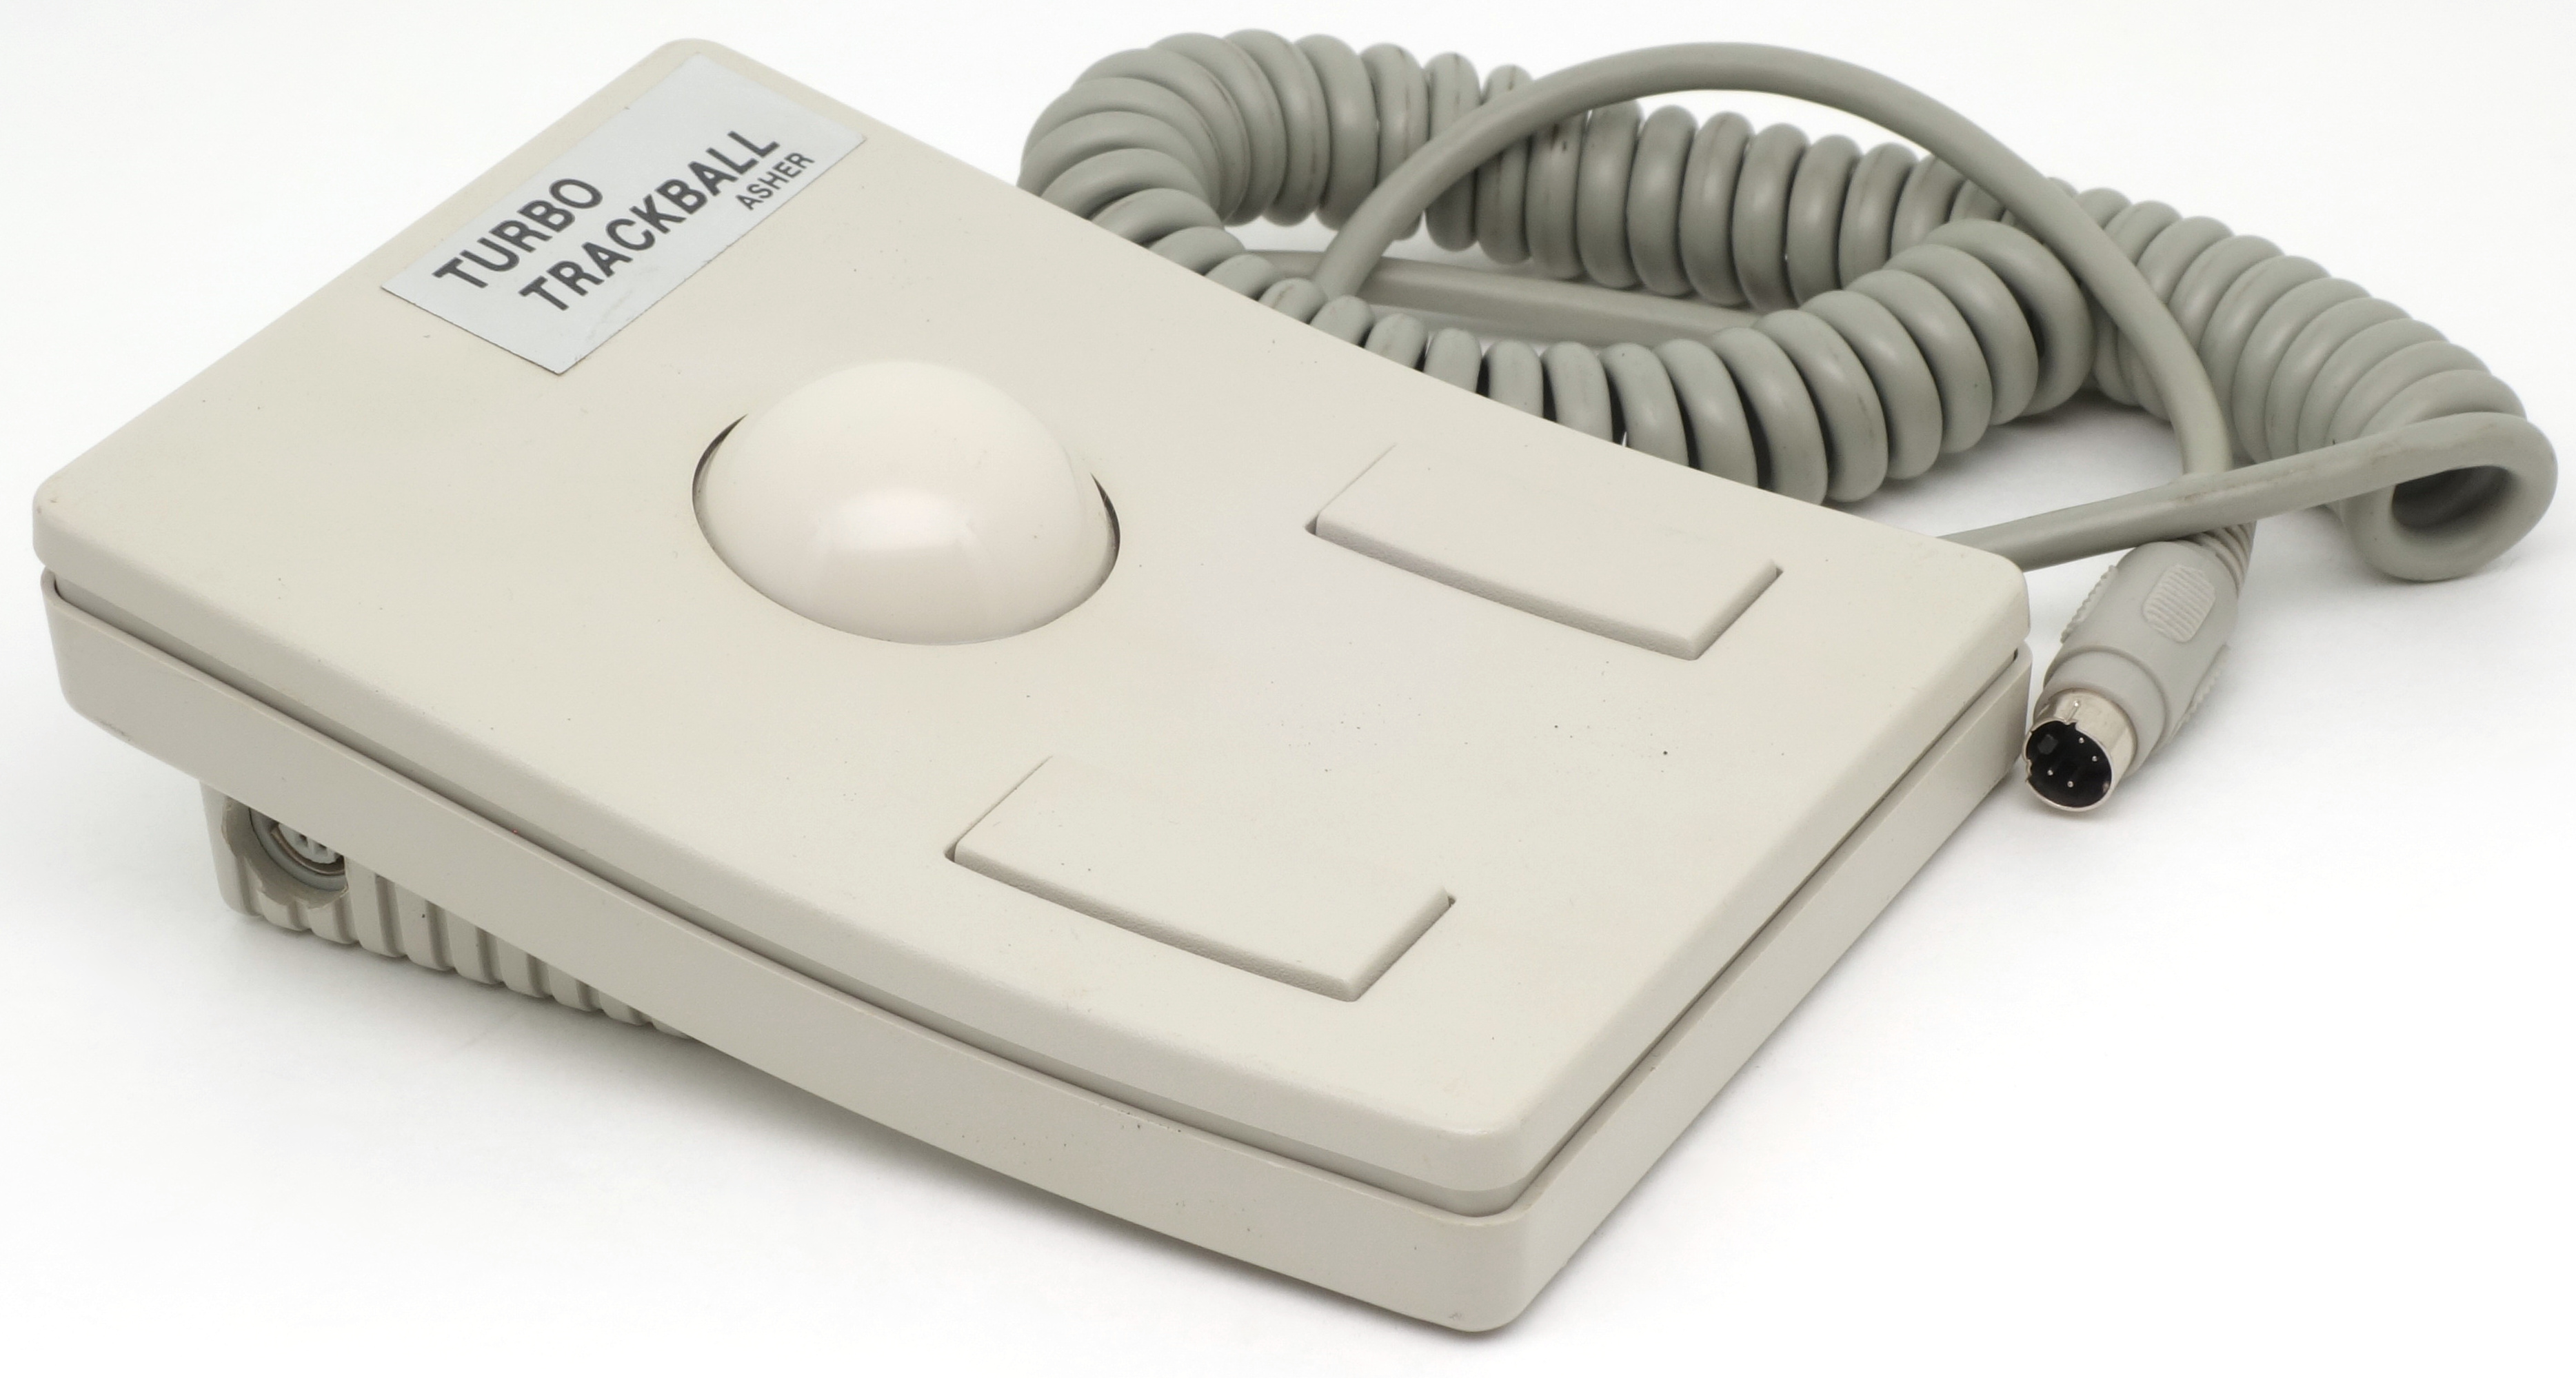
\includegraphics[scale=0.58]{1988_asher_turbo_trackball/pic_60.jpg}
    \caption{Внешний вид трекбола Asher Turbo}
    \label{fig:AsherPic}
\end{figure}

В отличие от классического вида моделей LX200, корпус Asher Turbo выполнен в корпусе, верхняя сторона которого имеет наклон в сторону пользователя и слегка вогнута, повторяя профиль компьютерных клавиатур того времени (рис. \ref{fig:AsherTopBottom}). Две прямоугольные кнопки, расположенные перед шаром с ближней к пользователю стороны "--- плоские, незначительно выступающие из корпуса, с большой площадью, выгодно сказывающейся на эргономике устройства. Левая кнопка работает в качестве главной кнопки мыши (а точнее, единственной, учитывая особенности экосистемы Apple), а правая "--- в качестве <<защелки>> перетаскивания. Нажатие кнопки-защёлки программно фиксирует главную кнопку трекбола в нажатом положении, а повторное нажатие любой из кнопок отключает данный режим.

Производитель позиционировал этот трекбол как <<универсальное, надежное, простое в использовании и очень точное устройство для сложных настольных издательских работ, графики, CAD/CAM и многих других приложений>>. В частности, подчеркивалось, что вся реклама этого трекбола, включая иллюстрации, была подготовлена к опубликованию на компьютере с использованием трекбола Asher Turbo \cite{turbo}.

\begin{figure}[h]
    \centering
    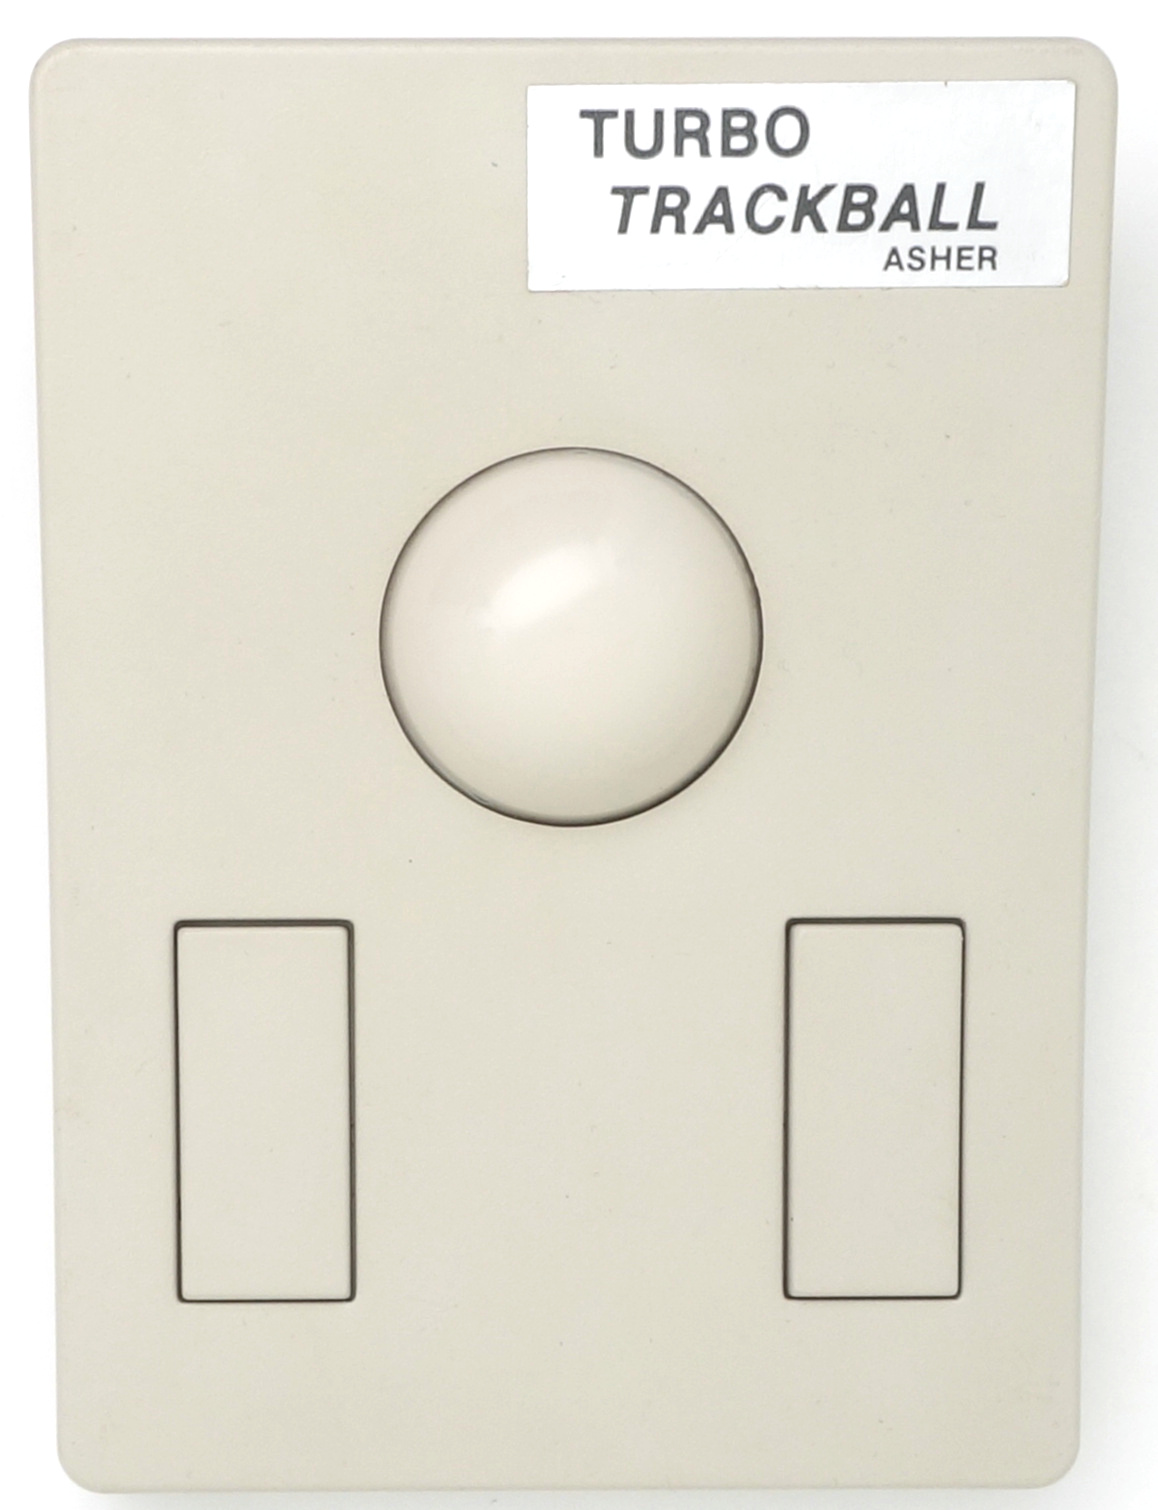
\includegraphics[scale=0.6]{1988_asher_turbo_trackball/top_15.jpg}
    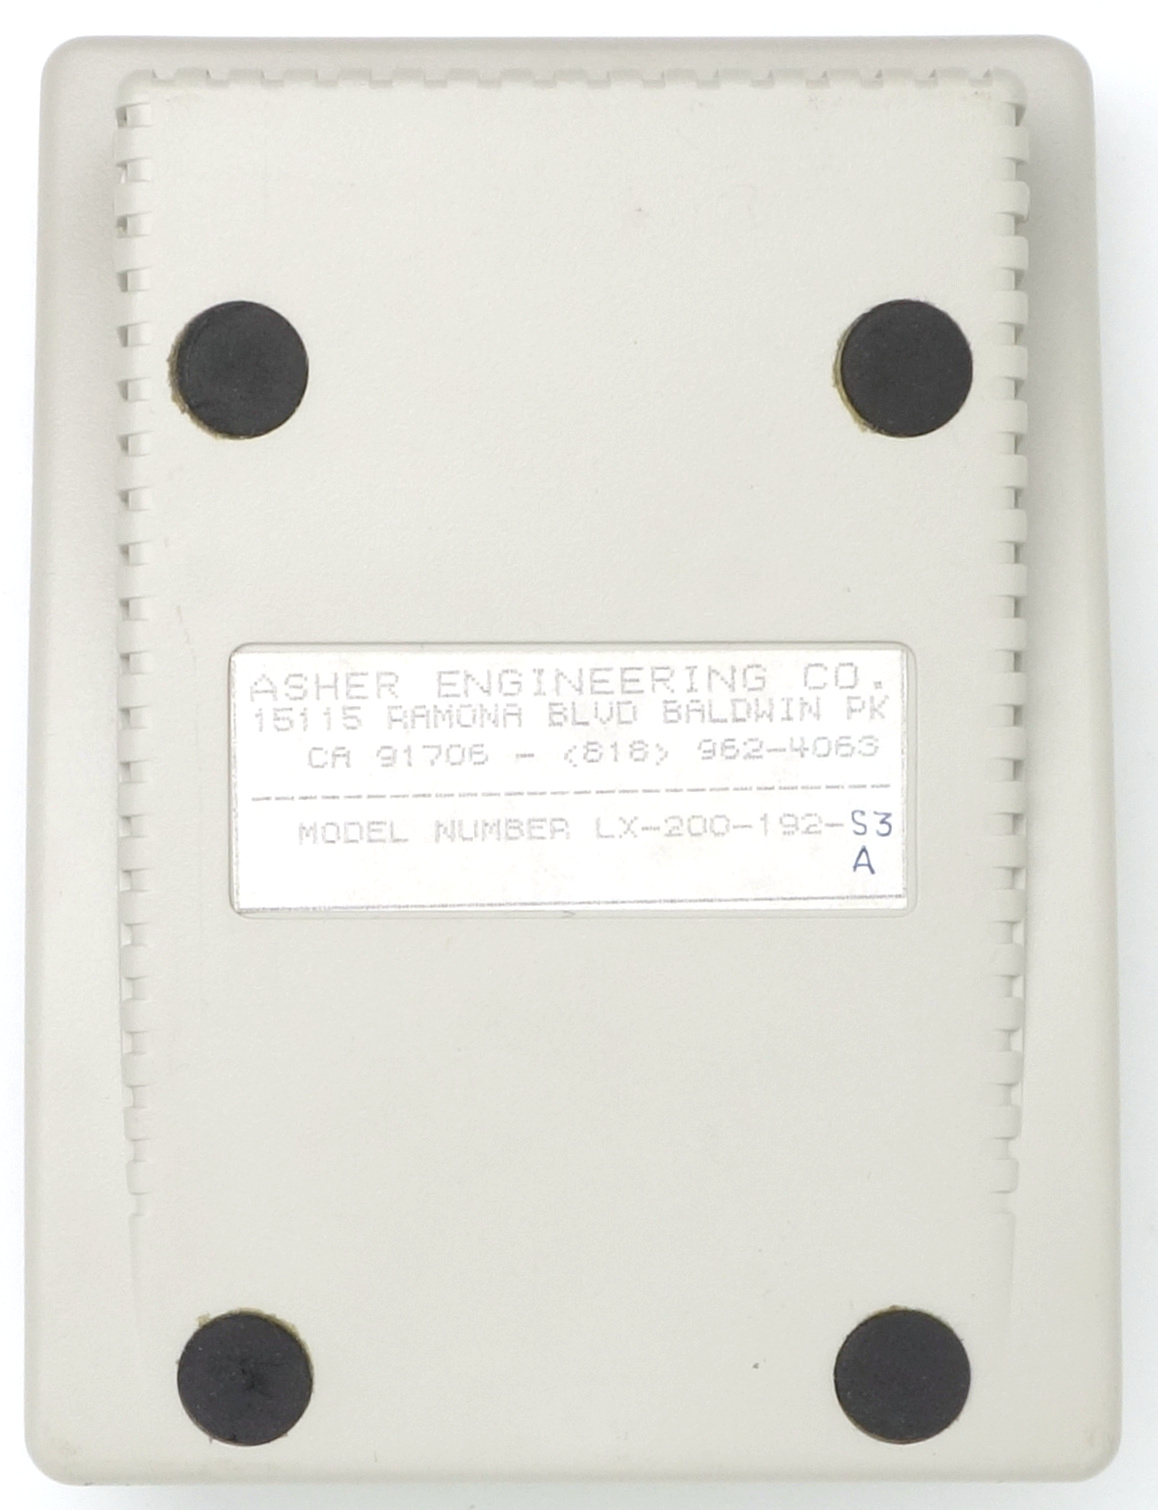
\includegraphics[scale=0.6]{1988_asher_turbo_trackball/bottom_15.jpg}
    \caption{Asher Turbo trackball, вид сверху и снизу}
    \label{fig:AsherTopBottom}
\end{figure}

Размеры трекбола меньше традиционных моделей LX200, поскольку диктуются габаритами компьютерной клавиатуры, для которой трекбол должен быть функциональным продолжением, находясь сбоку от неё. В целом, такое положение должно создавать достаточно комфортные условия для работы (рис. \ref{fig:AsherSize}).

Рекламные материалы подчеркивали преимущества трекбола Asher в сравнении с двумя моделями приблизительно того же форм-фактора "--- трекболами Abaton ProPoint и Kensington Turbo Mouse: отмечалось, что он обладает большей разрешающей способнсотью, обеспечивающей более точное управление курсором (250 CPI против 200 CPI у конкурентов), а также компактным низкопрофильным эргономичным корпусом. В отличие от оптомеханической схемы, используемой в трекболах Abaton и Kensington, фирма Asher отмечала собственный уникальный <<запатентованный высокотехнологичный энкодер, используемый также в сложных аэрокосмических приборах самолетов, ракет, торпед, гироскопов и космических челноков>> \cite{turbo}.

\begin{figure}[h]
    \centering
    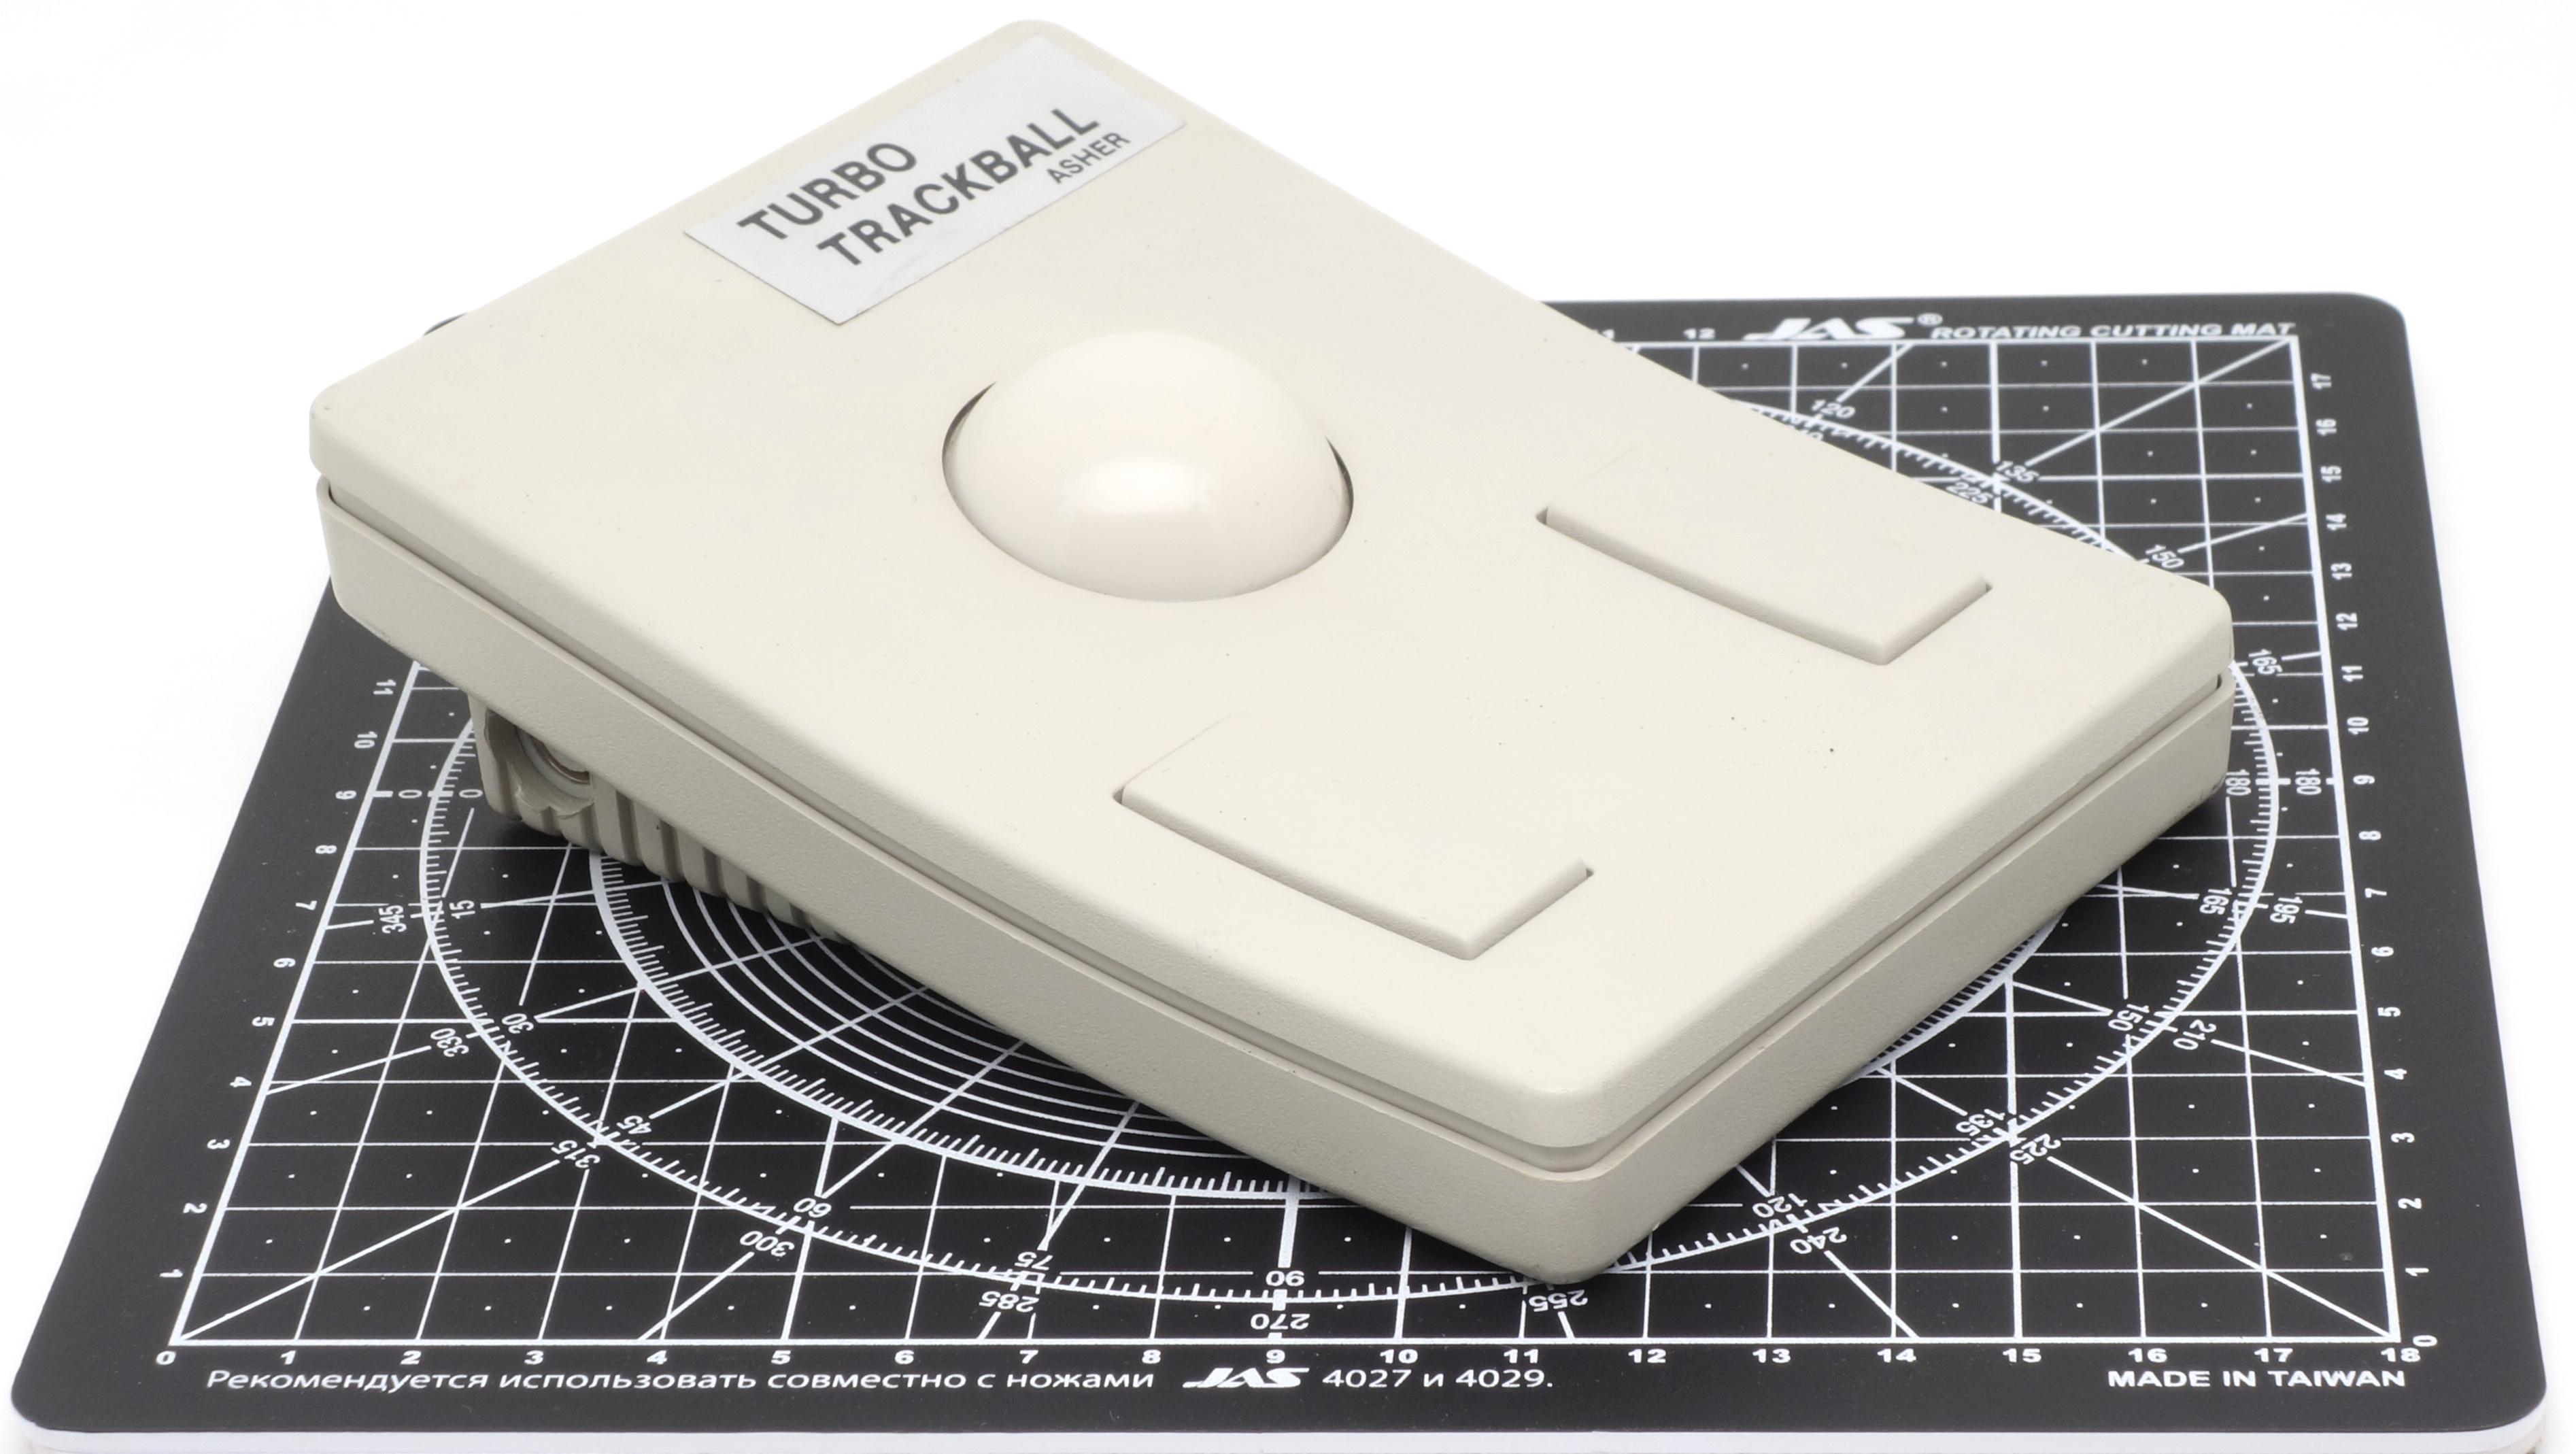
\includegraphics[scale=0.58]{1988_asher_turbo_trackball/size_30.jpg}
    \caption{Трекбол Asher Turbo на размерном коврике с шагом сетки 1 см}
    \label{fig:AsherSize}
\end{figure}

Трекбол симметричен, и в зависимости от того, правша пользователь или левша, он может расположить устройство слева или справа от клавиатуры. В рекламе упоминается наличие вариантов для правой и левой руки \cite{turbo}, но, учитывая отсутствие аппаратного переключателя, а также то, что ни долгое, ни одновременное нажатие кнопок не выполняют переключение, под <<вариантами>>, вероятно, понимаются варианты трекбола, то есть было необходимо покупать трекбол для нужной руки. В любом случае, в рабочем положении пользователю предлагается поместить указательный, средний пальцы на шар, а большой палец (и, возможно, мизинец) на кнопки мыши (рис. \ref{fig:AsherHand}). При этом в отличие от традиционных трекболов LX200, запястье опирается на поверхность стола, как при работе с клавиатурами компьютеров Macintosh.

\begin{figure}[h]
    \centering
    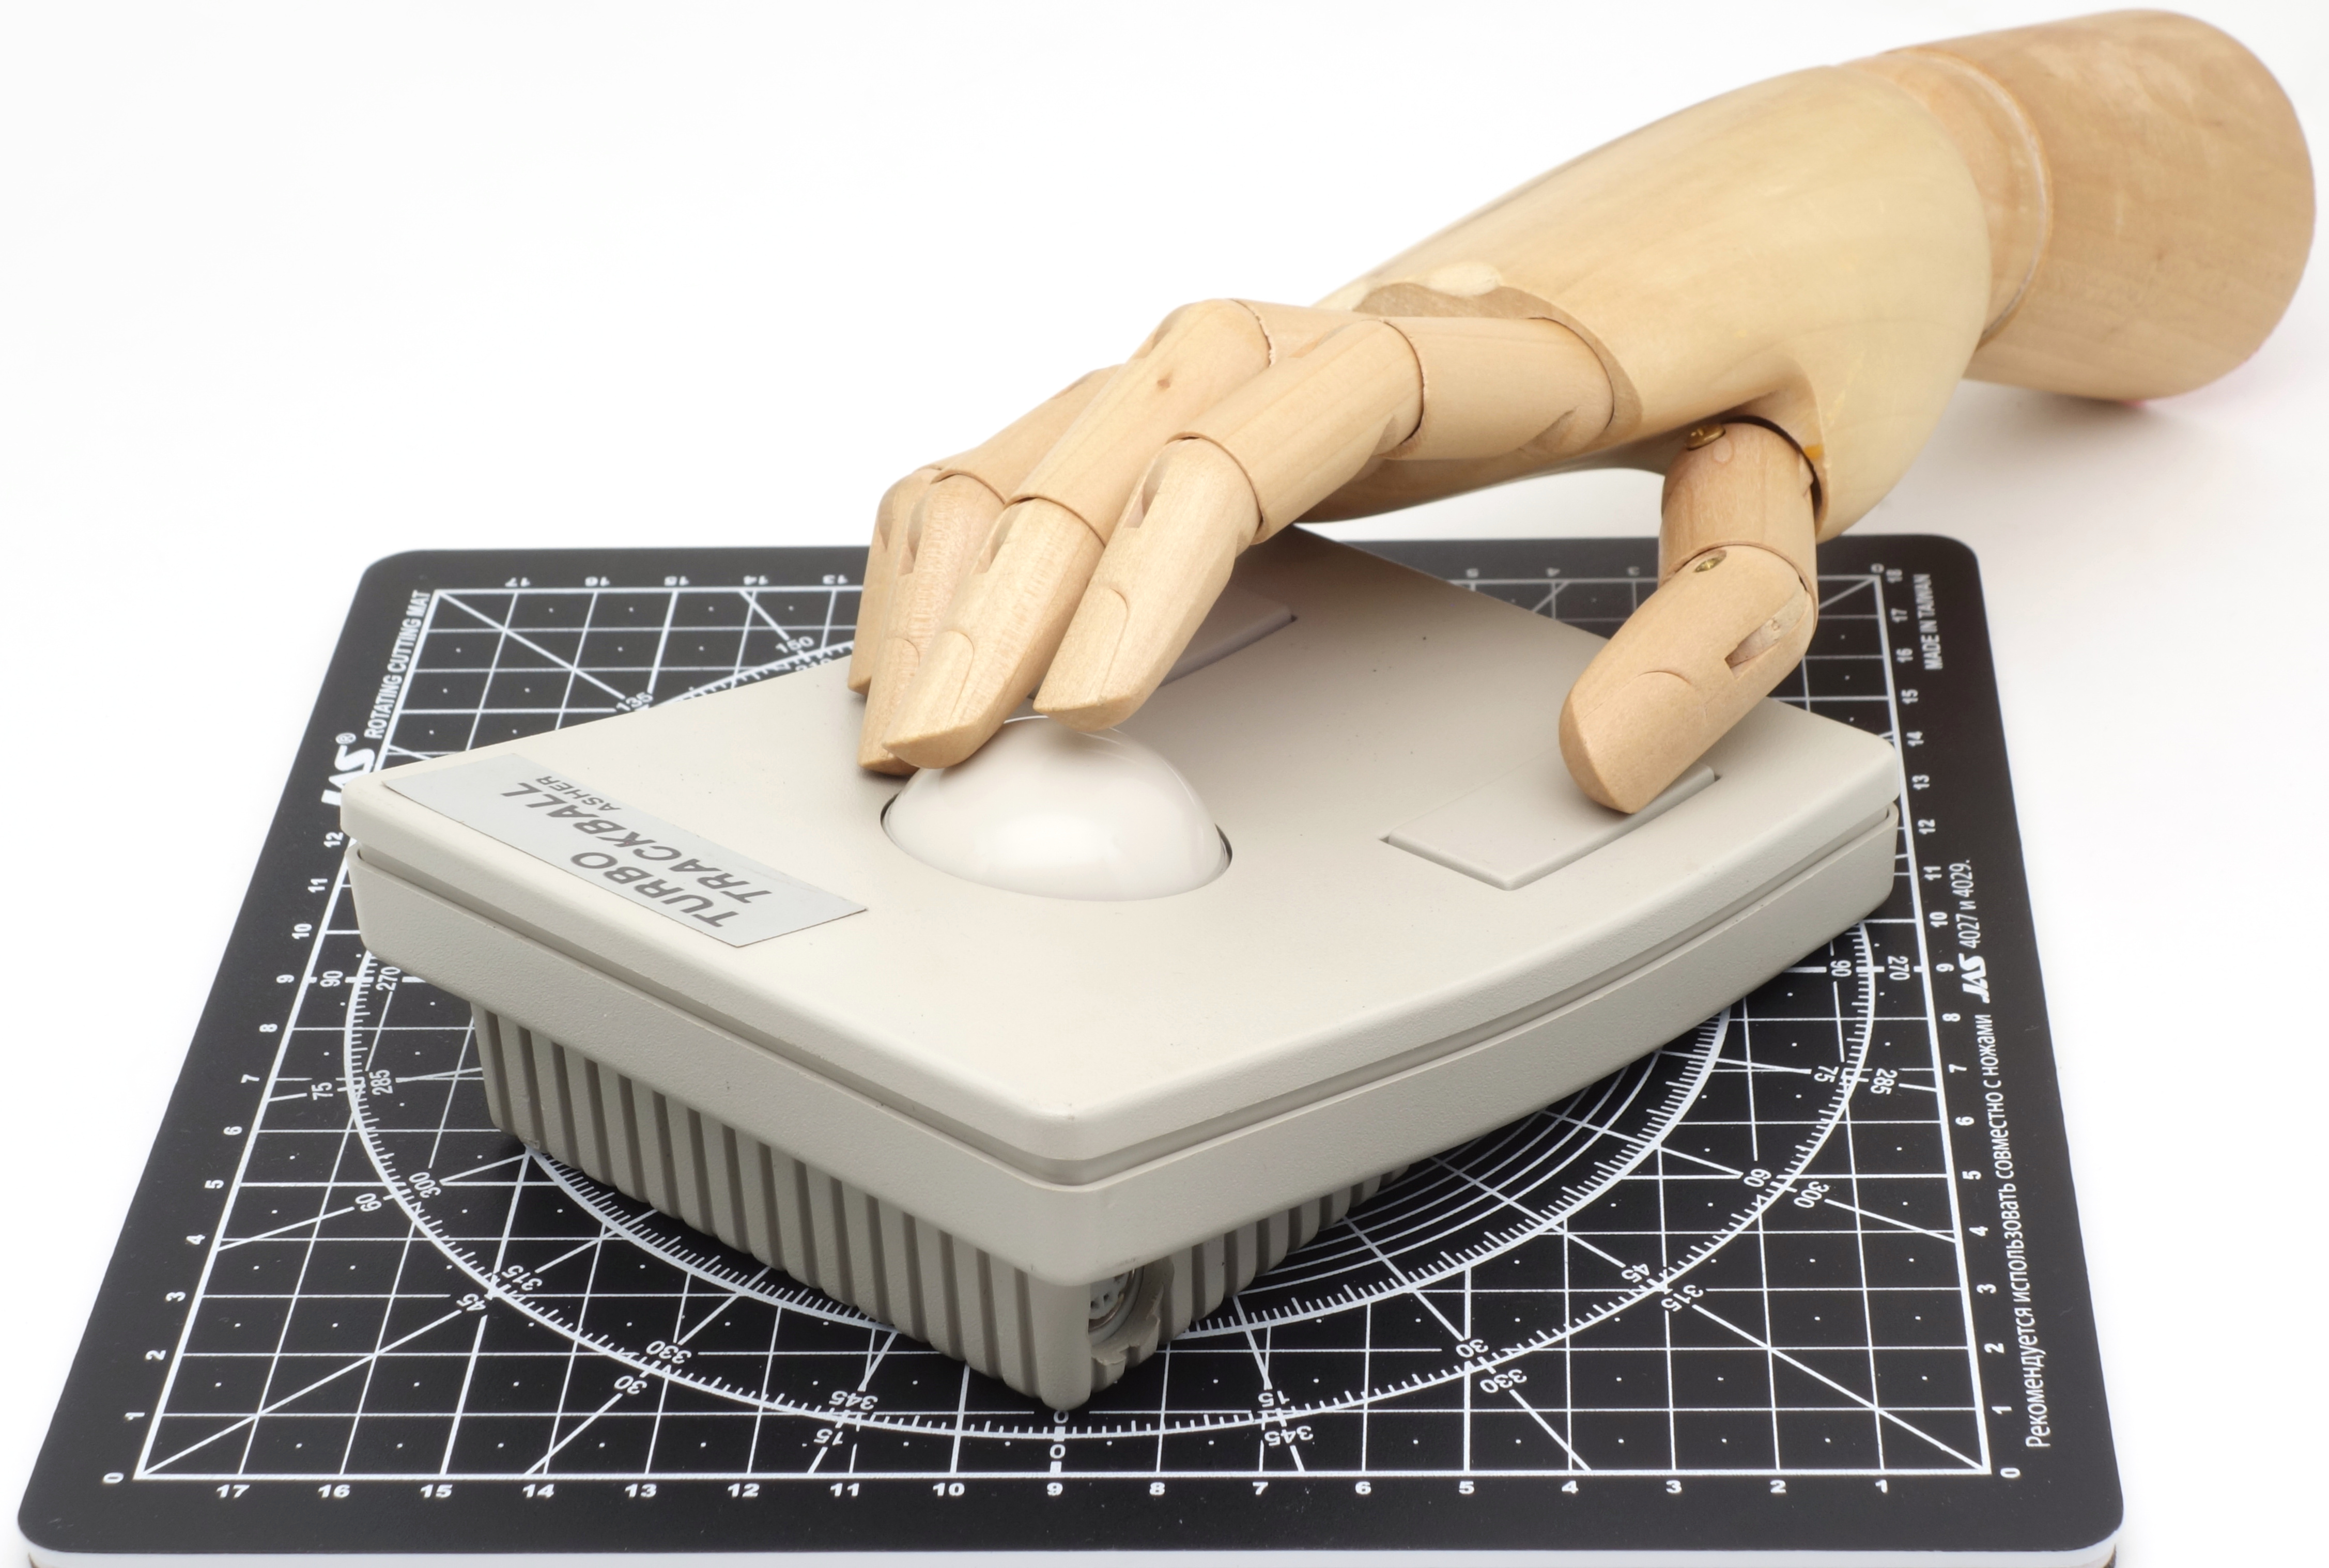
\includegraphics[scale=0.5]{1988_asher_turbo_trackball/hand_30.jpg}
    \caption{Трекбол Asher Turbo в комплекте с моделью руки человека}
    \label{fig:AsherHand}
\end{figure}

Внутреннее устройство данного трекбола показано на рис. \ref{fig:AsherInside}. В рекламе Asher Turbo Trackball подчеркивалось, что в отличие от конкурентов компания обладала собственным производством, и фотографии наглядно это демонстрируют: вместо традиционного литья, многие элементы вы полнены с помощью механической обработки (фрезеровки, сверления и т.д.) и пайки. Кроме того,  производитель отдает заметное предпочтение композитным материалам, традиционно используемым для изготовления печатных плат, таким как стеклотекстолит и гетинакс (по виду отдельных деталей можно предположить, что как раз из каких-то печатных плат они и были вырезаны). Наконец, <<запатентованный высокотехнологичный энкодер>> \cite{turbo} представляет собой обычный диск механичекого энкодера, накрытый сверху пластмассовой коробочкой, затрудняющей проникновение мусора (при этом его конструкция не настолько герметична и заметно менее технологична по сравнению, например, с закрытыми механическими энкодерами фирмы ALPS Electric, используемыми в ранних моделях мышей Microsoft, IBM и некоторых других компаний).

Очевидно, изготовление столь самобытной конструкции требовало существенного количества ручных операций, поэтому трекбол выпускался не слишком большими партиями.
Использование механического энкодера вместо оптомеханики было вероятно нацелено на удешевление устройства. В отличие от quadLYNX и других трекболов LX200 производства Honeywell, аналогичные изменения коснулись и других элементов механического узла: вместо подшипников и валов из нержавеющей стали использованы пластиковые ролики на металлической оси и опоры, вырезанные из композитного материала, одновременно играющие роль втулок. В качестве отличительной особенности можно отметить опору шара из шести стальных шариков, расположенных по кругу непосредственно в пазах на печатной плате.

\begin{figure}[h]
    \centering
    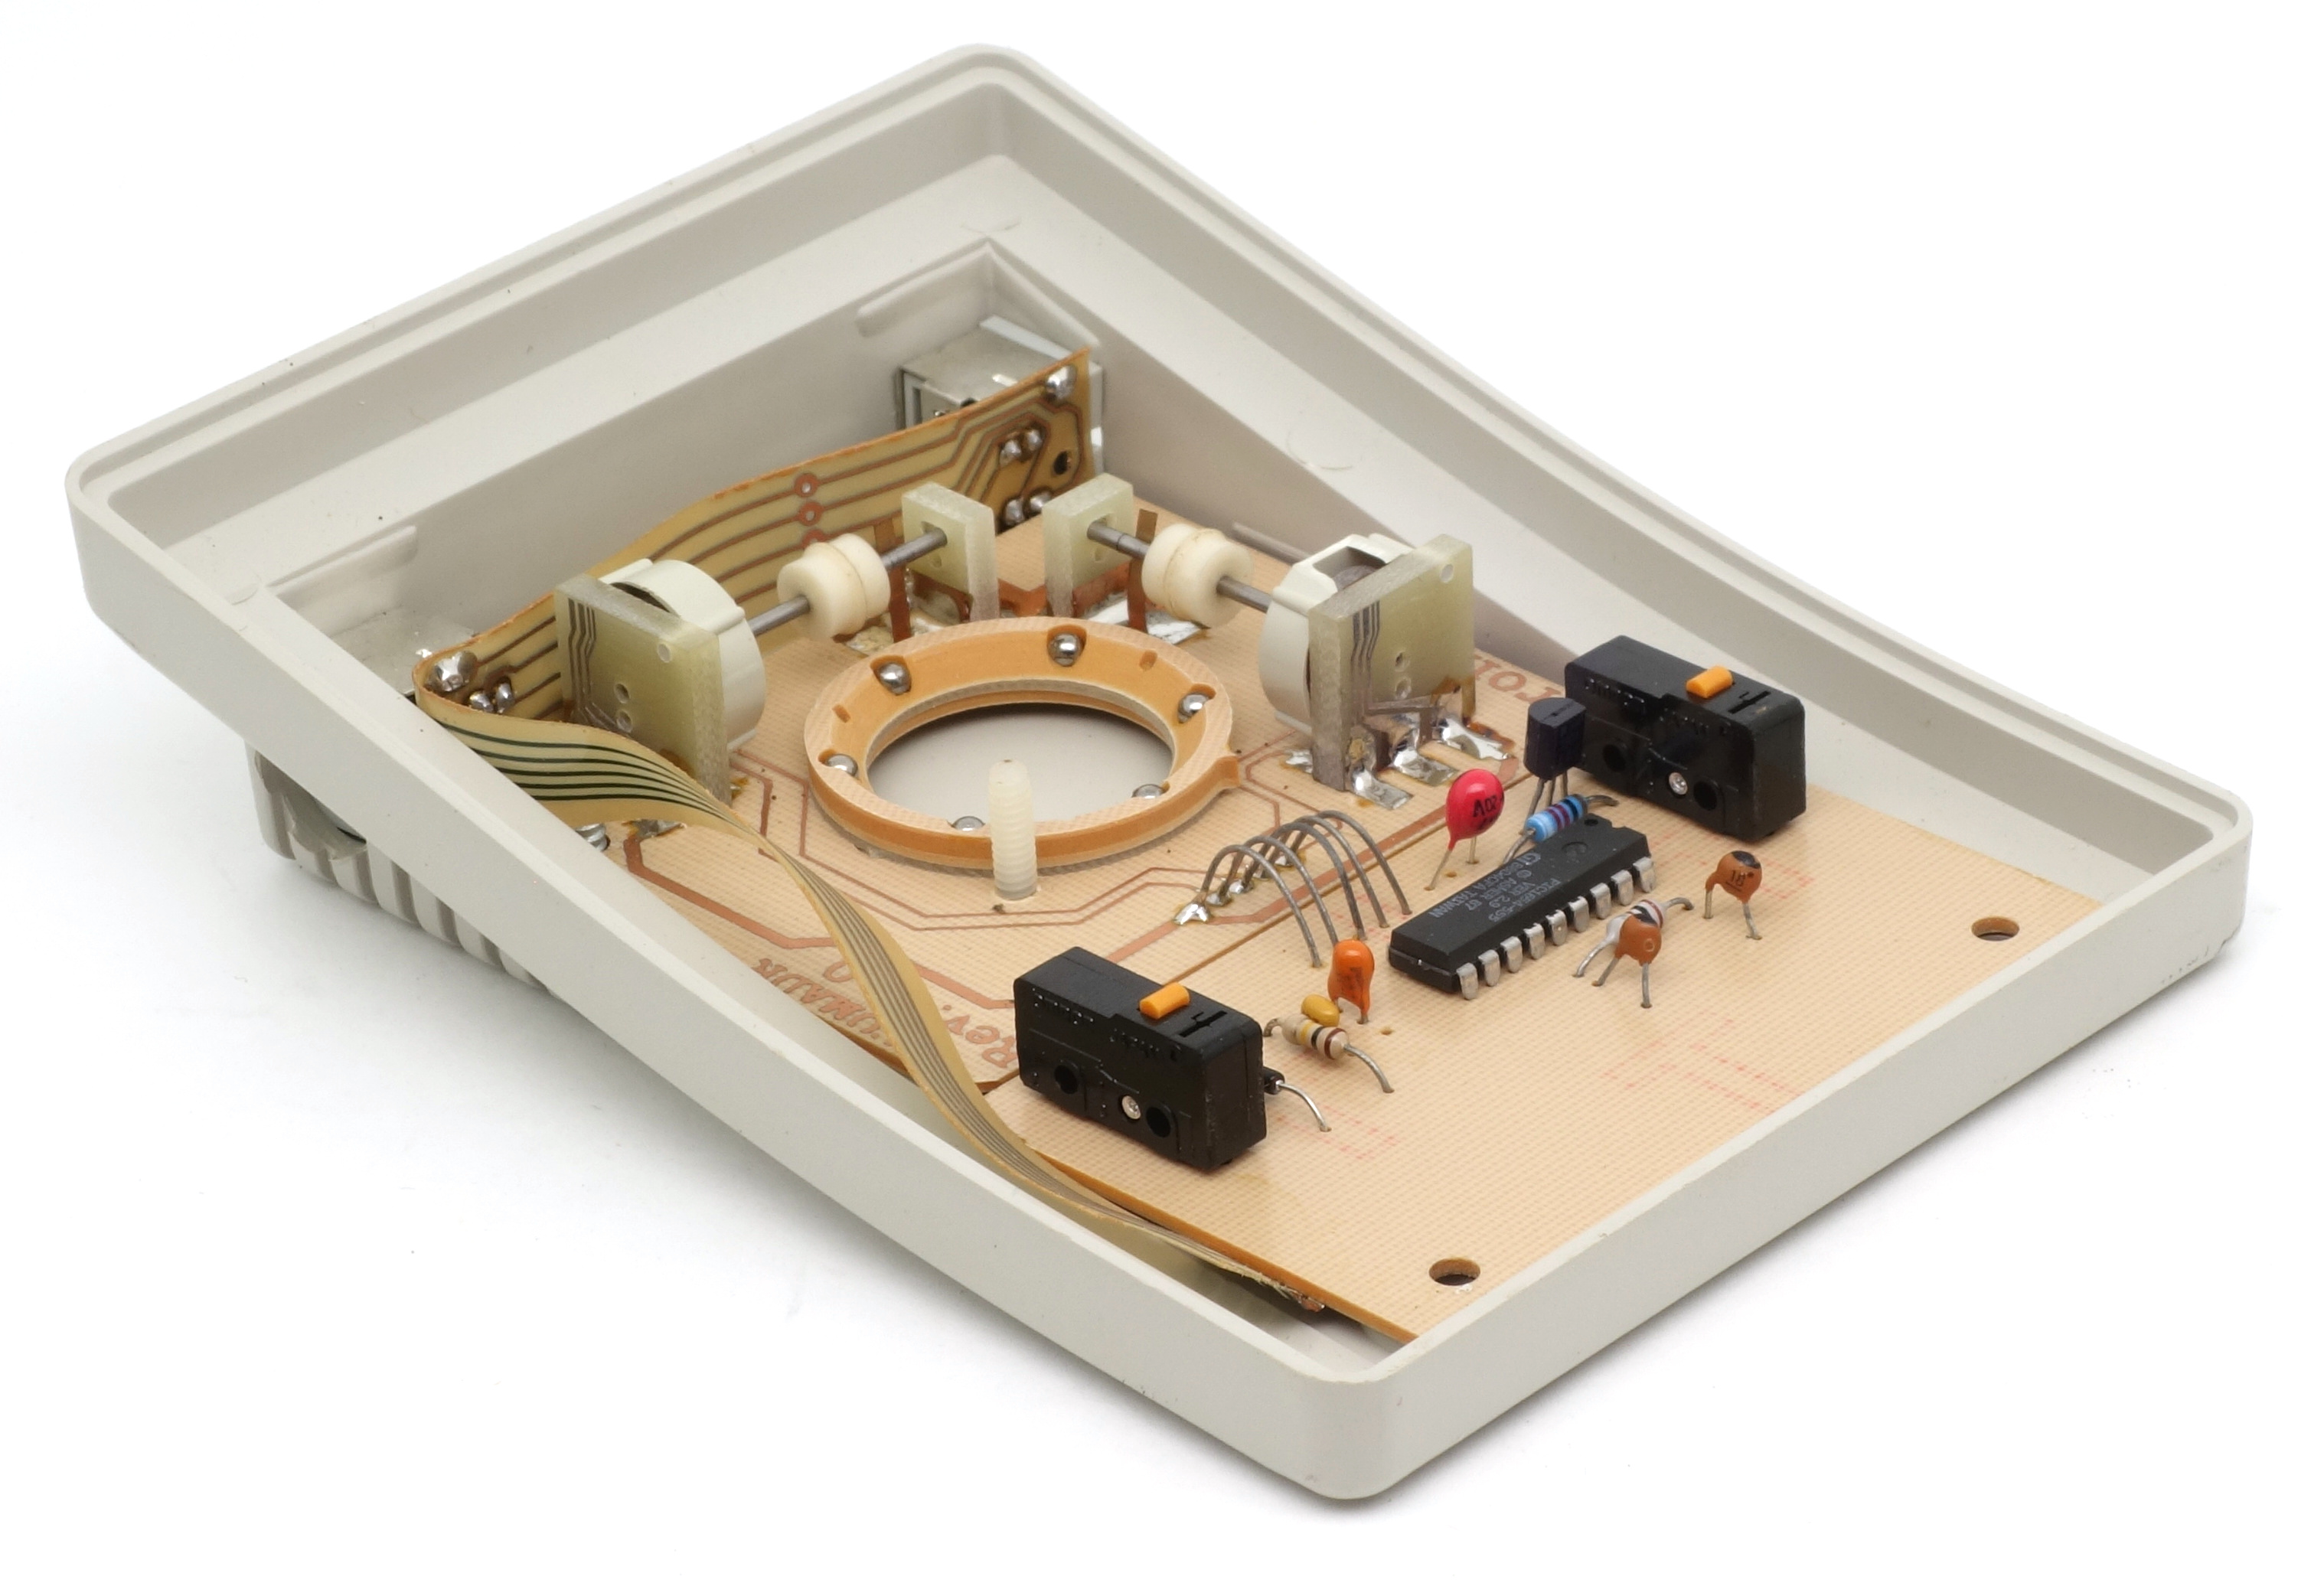
\includegraphics[scale=0.7]{1988_asher_turbo_trackball/inside_60.jpg}
    \caption{Asher Turbo trackball в разобранном виде}
    \label{fig:AsherInside}
\end{figure}

\begin{thebibliography}{9}
\bibitem {lx200} Disc Instruments LX200 \url{https://web.archive.org/web/20220501213039/https://forum.trackballs.eu/viewtopic.php?f=17&t=16}
\bibitem {honeywell} Try the new quadLYNX Trackball // Macworld, August 1986. P. 155  \url{https://archive.org/details/eu_Macworld-1986-08_OCR/page/n155/mode/2up}
\bibitem {asher} Try the new quadLYNX Trackball // Macworld, January 1988. P. 212 \url{https://archive.org/details/macworld00unse_oel/page/212/mode/2up}
\bibitem {turbo} New Turbo Trackball from Asher // MacUser, February, 1988. P. 320 
\url{https://archive.org/details/MacUser8802February1988/page/n323/mode/2up}
\end{thebibliography}
\end{document}

